

\documentclass[xcolor=x11names, compress]{beamer}

%% General document %%%%%%%%%%%%%%%%%%%%%%%%%%%%%%%%%%
\usepackage{graphicx}
\graphicspath{{./img/}}


\usepackage{xcolor}

\usepackage{tikz}
\usetikzlibrary{positioning, arrows}
\usetikzlibrary{decorations.fractals}
\tikzstyle{every picture}+=[remember picture]
\tikzstyle{na} = [baseline=-.5ex]

\usepackage{pgfplots}
\pgfplotsset{compat=newest}
\usepgfplotslibrary{units}
\usepgfplotslibrary{external}
\usetikzlibrary{pgfplots.external}
% \tikzset{external/system call={latex \tikzexternalcheckshellescape 
% -interaction=batchmode -jobname "\image" "\texsource";
% dvips -o "\image".ps "\image".dvi;
% ps2eps "\image.ps"}}
% \tikzset{external/force remake}
\tikzexternalize[prefix=tikz/external/]



\usepackage{filemod}
\newcommand{\includetikz}[2]{%
  \tikzsetnextfilename{#2}%
  \filemodCmp{#1#2.tikz}{#1external/#2.pdf}%
    {\tikzset{external/remake next}}{}%
  \input{#1#2.tikz}%
}




\pgfplotsset{
  /pgfplots/scatter legend/.style={
    /pgfplots/legend image code/.code={\draw[##1,yshift=-0.1em] plot coordinates {
      (-0.1em, 0.1em)
      (0.2em, 0.45em)
      (0.3em, -0.05em)
      (0.6em, 0.3em)
    };},
    rounded corners=1.5pt,
  },
}


\usepackage{filecontents, anyfontsize, textcomp, siunitx}

\usepackage[super]{nth}


%%%%%%%%%%%%%%%%%%%%%%%%%%%%%%%%%%%%%%%%%%%%%%%%%%%%%%


%% Beamer Layout %%%%%%%%%%%%%%%%%%%%%%%%%%%%%%%%%%
%\useoutertheme[subsection=false,shadow]{miniframes}
\useoutertheme[subsection=false,shadow]{miniframes}
\usepackage{etoolbox}
\makeatletter
\patchcmd{\slideentry}
{\advance\beamer@xpos by1\relax}{}{}{}
\def\beamer@subsectionentry#1#2#3#4#5{\advance\beamer@xpos by1\relax}
\makeatother

%\setbeamertemplate{footline}{%
%\begin{beamercolorbox}{section in head/foot}
%    \color{gray}\vskip2pt~ \insertsection\hfill\insertpagenumber{} %
%    / \insertpresentationendpage{} ~\vskip2pt
%\end{beamercolorbox}
%}

\setbeamertemplate{footline}{%
\begin{beamercolorbox}{0}
    \color{black}\vskip2pt~ \hfill\insertframenumber{} \hspace{10pt} \vspace{3pt} ~\vskip2pt
\end{beamercolorbox}
}

\setbeamertemplate{navigation symbols}{}

\useinnertheme{default}
\usefonttheme{structuresmallcapsserif} % could be default, serif, structurebold, professionalfonts, structureitalicserif or structuresmallcapsserif
\usepackage{palatino}

\setbeamerfont{title like}{shape=\scshape}
\setbeamerfont{frametitle}{shape=\scshape}

\setbeamercolor*{lower separation line head}{bg=DeepSkyBlue4} 
\setbeamercolor*{normal text}{fg=black,bg=white} 
\setbeamercolor*{alerted text}{fg=red} 
\setbeamercolor*{example text}{fg=black} 
\setbeamercolor*{structure}{fg=black} 
 
\setbeamercolor*{palette tertiary}{fg=black,bg=black!10} 
\setbeamercolor*{palette quaternary}{fg=black,bg=black!10} 

\renewcommand{\(}{\begin{columns}}
\renewcommand{\)}{\end{columns}}
\newcommand{\<}[1]{\begin{column}{#1}}
\renewcommand{\>}{\end{column}}
%%%%%%%%%%%%%%%%%%%%%%%%%%%%%%%%%%%%%%%%%%%%%%%%%%


\AtBeginSection[]
{
  {
  \tikzexternaldisable
  \setbeamertemplate{footline}{}
  \begin{frame}[noframenumbering]{}
    \vfill
    \begin{center}
    \rmfamily \LARGE \insertsection
    \end{center}
        \begin{tikzpicture}[scale=0.1]
        % finalsectionnumber * delta = 115
        \pgfmathsetmacro\res{\insertsectionnumber * 28.75}
    \fill [lightgray] (9cm,0cm) rectangle (115cm,1cm);
    \fill [black] (9cm, 0cm) rectangle (\res cm,1cm);
    \end{tikzpicture}
    \vfill
  \end{frame}
  \tikzexternalenable
  }
}

\definecolor{lightgray}{gray}{0.75}
\definecolor{darkgreen}{RGB}{50,200,10}
\newcommand{\ver}[1]{\texttt{\textbf{#1}}}
\everymath{\displaystyle}
\newcommand{\btVFill}{\vskip0pt plus 1filll}
\DeclareSIUnit\nat{nat}


\usepackage{listings}
\lstset{
  language=Python,
  showstringspaces=false,
  formfeed=newpage,
  tabsize=4,
  commentstyle=itshape,
  morekeywords={models, lambda, forms}
}

\begin{document}


%%%%%%%%%%%%%%%%%%%%%%%%%%%%%%%%%%%%%%%%%%%%%%%%%%%%%%
%%%%%%%%%%%%%%%%%%%%%%%%%%%%%%%%%%%%%%%%%%%%%%%%%%%%%%
\begin{frame}[plain]
  \title{ {\fontsize{10}{1}\selectfont An Unexpected Discrepancy in a Well-known Problem:} \\ \vspace{3pt} {\fontsize{14}{1}\selectfont \bfseries Kraskov Estimators  Applied to \\ \vspace{-3pt} Spiking Neural Networks} \\ }
\subtitle{ ~ }
\date{}
\vspace{5pt}
\titlepage
\vfill
\begin{center}

% {
% \tikzexternaldisable
%   \begin{tikzpicture}
%     \tikzstyle{inhib}=[-*, semithick, opacity=0.8, black!20!blue]
%     \tikzstyle{excit}=[-stealth', shorten >=1pt, opacity=0.8, semithick, black!20!blue]
%     \tikzstyle{synap}=[-stealth', gray!90!white, dashed]
%     \def\neuronR{1.6cm};
%     \def\netR{3cm}
% 
%       % \node[circle, fill=purple!50!black, opacity=0.2, minimum size=1.7*\neuronR] (INC) at (0:0cm) {};
%     \node[circle, thick, fill=blue!50!green] (titleInhib) at (0,0) {};
% 
%       \node[circle, fill=blue!60!green, opacity=0.4, minimum size=\neuronR] (titleExcit) at  (2,0) {};
%       \draw[inhib] (titleInhib) -- (titleExcit);
% 
%     \path[excit, bend left] (titleExcit) edge (titleInhib);
% 
%   \end{tikzpicture}
% 
% \tikzexternalenable
% }

  ~ \\
  
  \vfill
  {\large Pedro Mediano}\\ \vspace{-8pt}
  {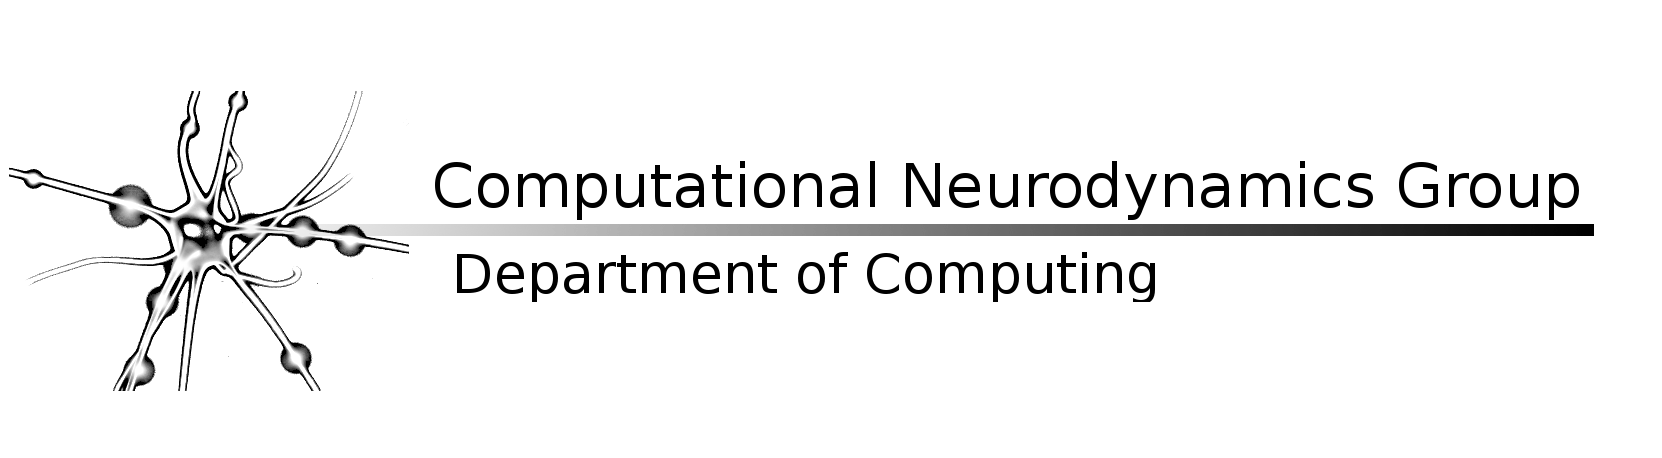
\includegraphics[width=0.7\textwidth]{logo3.png}}\\ \vspace{-10pt}


\ver{pmediano@ic.ac.uk} \hspace{20pt} Imperial College, London
\end{center}
\end{frame}


%%%%%%%%%%%%%%%%%%%%%%%%%%%%%%%%%%%%%%%%%%%%%%%%%%%%%%
%%%%%%%%%%%%%%%%%%%%%%%%%%%%%%%%%%%%%%%%%%%%%%%%%%%%%%
\section{ \scshape Introduction}
\subsection{Introduction}
\begin{frame}{Introduction}
  \bigskip

  \begin{itemize}
    
    \item One of the goals of complex systems research is to understand
    \textbf{collective behaviour}.

    \vfill
    \pause
    \item We need robust tools and solid \textbf{statistical tests}.

  \end{itemize}


  \btVFill


\end{frame}


%%%%%%%%%%%%%%%%%%%%%%%%%%%%%%%%%%%%%%%%%%%%%%%%%%%%%%
%%%%%%%%%%%%%%%%%%%%%%%%%%%%%%%%%%%%%%%%%%%%%%%%%%%%%%
\begin{frame}{Why Python?}

  Why Python

\end{frame}


%%%%%%%%%%%%%%%%%%%%%%%%%%%%%%%%%%%%%%%%%%%%%%%%%%%%%%
%%%%%%%%%%%%%%%%%%%%%%%%%%%%%%%%%%%%%%%%%%%%%%%%%%%%%%
\begin{frame}[fragile]{Python basics}

\textbf{The import system}

\begin{itemize}
	\item Often the definitions (e.g. functions) we want to use might be stored in a different script called \textit{module}.
	\item In order to use definitions from other modules we need to import these modules at the beginning of our script.
	\item This is done via the command \textit{import} 
			\begin{lstlisting}[xleftmargin=.2\textwidth]
				import numpy 
			\end{lstlisting}
	\item If the name of the module is long we can set a new abbreviation for it
			\begin{lstlisting}[xleftmargin=.2\textwidth]
				import numpy as np
			\end{lstlisting}
	\item We can also load specific definitions:
			\begin{lstlisting}
				from numpy import array / from numpy import * 
			\end{lstlisting}
\end{itemize}



 % Python basics (import, tabs, colons, classes)
\end{frame}


%%%%%%%%%%%%%%%%%%%%%%%%%%%%%%%%%%%%%%%%%%%%%%%%%%%%%%
%%%%%%%%%%%%%%%%%%%%%%%%%%%%%%%%%%%%%%%%%%%%%%%%%%%%%%

\begin{frame}[fragile]{Python basics}
\textbf{Classes}
\begin{itemize}
\item Classes are blueprints for creating objects
\item Classes can contain functions that are applied to objects from that class
\end{itemize}

\begin{lstlisting}[xleftmargin=.2\textwidth]
class Shape:
    def __init__(self, x , y):
        self.x = x
        self.y = y

    def area(self):
        return self.x * self.y

rectangle = Shape(100, 45)
print rectangle.area()
\end{lstlisting}
\end{frame}

%%%%%%%%%%%%%%%%%%%%%%%%%%%%%%%%%%%%%%%%%%%%%%%%%%%%%%
%%%%%%%%%%%%%%%%%%%%%%%%%%%%%%%%%%%%%%%%%%%%%%%%%%%%%%

\begin{frame}[fragile]{Python basics}
\textbf{Indentations in python}
\begin{itemize}
\item Indentations mark the blocks of code within script 
\item Each line of a block must be indented by the same amount
\end{itemize}

\begin{lstlisting}[xleftmargin=.2\textwidth]
if (some condition):
    if (another condition):
        do_something(fancy)
else:
    do_something(different)
\end{lstlisting}

\begin{itemize}
\item Mind that beginnings of blocks are indicated with a colon ":"
\end{itemize}

\textbf{0 - indexing}
\begin{itemize}
\item The index of the first element in python is 0
\item Tip: "-1" refers to the last element 
\end{itemize}
\end{frame}

%%%%%%%%%%%%%%%%%%%%%%%%%%%%%%%%%%%%%%%%%%%%%%%%%%%%%%
%%%%%%%%%%%%%%%%%%%%%%%%%%%%%%%%%%%%%%%%%%%%%%%%%%%%%%

\begin{frame}[fragile]{Moving from Matlab to Python}
\textbf{Replacing Matlab with python}
\begin{itemize}
\item Overall Matlab and python are very similar in terms of syntax
\item \textbf{Similarities:} 
	\begin{enumerate}
	\item Both are \textit{dynamically typed} (every variable can contain data of any type)
	\item Both are \textit{interpreted}, they do not need to be compiled
	\end{enumerate}
\item \textbf{Differences}
	\begin{enumerate}
	\item Python files can contain unlimited functions that can all be accessed 
	\item Python does not have a matrix engine but there are useful packages with similar functionalities
		\begin{itemize}
		\item \textbf{Numpy}: enables basic matrix arithmetics on arrays
		\item \textbf{Scipy}
		\item \textbf{Matplotlib}: plotting
		\end{itemize}
	\end{enumerate}
\end{itemize}
\end{frame}

%%%%%%%%%%%%%%%%%%%%%%%%%%%%%%%%%%%%%%%%%%%%%%%%%%%%%%
%%%%%%%%%%%%%%%%%%%%%%%%%%%%%%%%%%%%%%%%%%%%%%%%%%%%%%

\begin{frame}{Other}
  Moving from Matlab to Python
    Data structure comparison

  Python development tools (Spyder, atom, vim, pdb)
    Ubuntu access (registration)
    Create virtualenv and install jpype


  Tutorial links, exercises
\end{frame}
  

%%%%%%%%%%%%%%%%%%%%%%%%%%%%%%%%%%%%%%%%%%%%%%%%%%%%%%
%%%%%%%%%%%%%%%%%%%%%%%%%%%%%%%%%%%%%%%%%%%%%%%%%%%%%%
\begin{frame}{Live example}
  Go through IzNeuronDemo.py

\end{frame}



\end{document}

